\documentclass[10pt]{report}

\usepackage{amsmath}
\usepackage{amssymb}
\usepackage{array}
\usepackage{tabu}
\usepackage{lmodern}
\usepackage{graphicx}
\usepackage[space]{grffile}
\usepackage{subfigure}
\usepackage{longtable}
\usepackage[margin=1.0in]{geometry}
\renewcommand{\baselinestretch}{2.0}

\begin{document}
	\section{Introduction:}
	\subsection{Identifiability analysis: Definitions and Formulations}
	The identifiability of parameters in nonlinear models of physical processes can be classified into two categories: structural and practical identifiability. The effect of model structure and parameterization on the ability to infer true parameter values from experimental data is determined by the structural identifiability of the parameter. The effect of the available experimental data on the ability to estimate unique parameter values is determined by the practical identifiability of the parameter. Practical identifiability of a parameter is contingent upon the nature, quality and quantity of data available to estimate the parameter as opposed to the structure and parameterization of the model. The aforementioned distinction between practical and structural identifiability of parameters is illustrated in Figure. Thus, the identifiability of parameters in nonlinear models is dependent on the model structure, parameterization, and the quality and quantity of experimental data that is available for the purpose of estimation. 
	
	On the one hand, establishing the structural identifiability of parameters enables one to propose models that are not only appropriate representations of physical processes, but also are parameterized in such a way that the value of these parameters can be estimated. On the other hand, establishing practical identifiability of parameters in any model helps design experiments that are minimal, informative and useful for parameter estimation. 
	
	We can use a profile likelihood-based approach to determine the structural and practical identifiability of parameters in any any dynamic model. 
	
	We show how experimental design can have a meaningful impact on parameter identification and estimation in Figure \ref{fig:edwithpl}.
	
	\begin{figure}[!tbhp]
		\centering{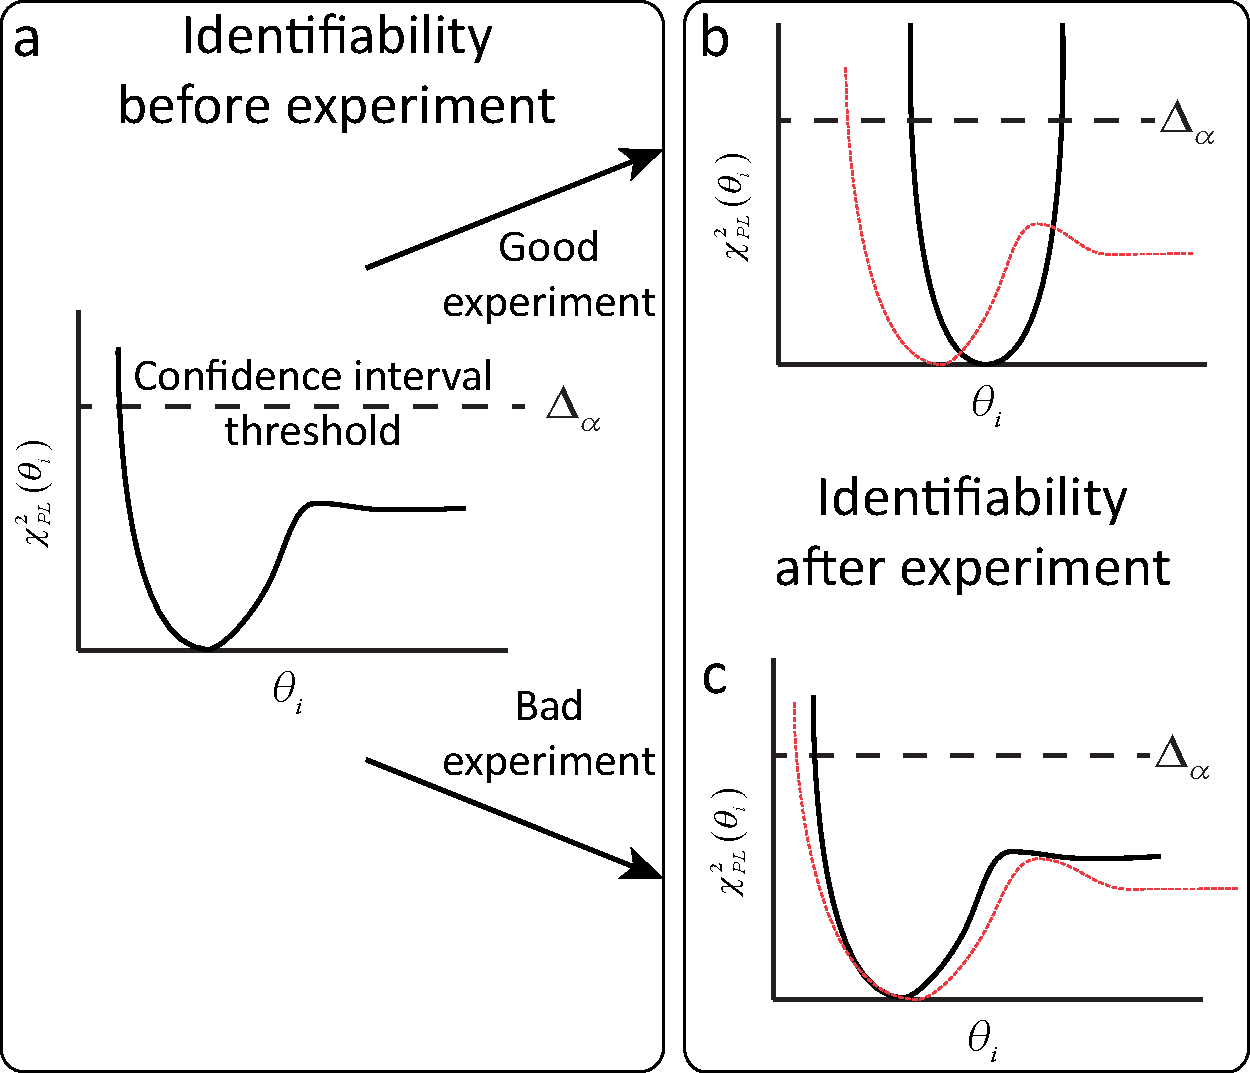
\includegraphics[width=.6\textwidth,height=.6\textheight,keepaspectratio]{figures/ed_with_pl}}
		\caption{Cartoon illustrating the utility of identifiability analysis for experimental design. a) The profile likelihood of a practically non-identifiable parameter that needs to be estimated based on both good and bad experimental data. The changes in the profile likelihood of the parameter when estimated with b) good experimental data and c) bad experimental. The identifiability of the parameter does not change due to the poor quality/quantity of experiments.}\label{fig:edwithpl}
	\end{figure}
	
	\section{Methods:}
	We use a profile likelihood-based approach to establish structural and practical identifiability of parameters in nonlinear kinetic models of metabolism. Briefly, the approach seeks to establish the existence/non-existence of bounds in confidence intervals for the estimates of parameters in nonlinear models. The profile likelihood is calculated based on Equation \ref{eq:pl} for each parameter $\theta_i$ where $\chi^2(\theta_i)$ is given by Equation \ref{eq:chi2}.
	\begin{align}\label{eq:pl}
	\chi_{PL}^2(\theta_i) = \underset{\theta_{j\ne i}}{\mathrm{min}} \left[\chi^2(\theta)\right]
	\end{align}
	\begin{align}\label{eq:chi2}
	\chi^2(\theta) = \sum_{k=1}^{m}\sum_{l=1}^{d}\left(\frac{y_{kl}^*-y_{kl}}{\sigma_{kl}^*}\right)^2
	\end{align}
	Equation \ref{eq:chi2} is typically used as the objective to be minimized in a typical parameter estimation problem where $y_{kl}^*$ is the available experimental time course data for each observable state $k$ at each $l$ time point. The difference between this data and the model estimates at these time points, $y_{kl}$ is weighted by the experimental error $\sigma_{kl}^*$. An algorithm to calculate $\chi_{PL}^2(\theta_i)$ based on Equation \ref{eq:pl} is given below.
	
	\subsubsection{Algorithm:}	
	\begin{enumerate}
		\item Start by solving the numerical optimization problem in Equation \ref{eq:pl} for a fixed value of $\theta_i$ to determine the initial point on the profile likelihood curve.
		\item Take an increasing/decreasing step $\theta_{step}$ in the direction of $\theta_i$.
		\item Re-optimize $\theta_{j\ne i}$ using Equation \ref{eq:pl}.
		\item Repeat the last two steps until a desired threshold $\Delta_{\alpha}$ is exceeded or a maximal amount of steps is reached.
	\end{enumerate}

	\subsubsection{Adaptive step change:}
	The increasing/decreasing steps in $\theta_i$ can be adapted to the shape of the profile likelihood curve that is encountered while running the above algorithm. Accordingly, the step $\theta_{step}$ should satisfy Equation \ref{eq:adaptivestep} below, where $\theta^{k-1}$ refers to parameter estimates obtained from iteration $k-1$ of the above algorithm, and $q\in \left[0,1\right]$.
	\begin{align}\label{eq:adaptivestep}
	\chi^2\left(\theta^{k-1}+\theta_{step}\right) - \chi^2(\theta^{k-1}) \approx q.\Delta_{\alpha}
	\end{align}
\end{document}